\chapter{Wstęp}
\label{ch:wstep}

Zanim przejdziesz dalej musisz odpowiedzieć sobie na bardzo ważną kwestię. Czy chcesz podczas pisania pracy dyplomowej ręcznie kontrolować, sprawdzać i~wciąż na nowo ustawiać takie rzeczy jak:

\begin{itemize}
	\item wielkość i~rodzaj czcionki,
	\item długość wcięcia akapitu,
	\item styl tytułów rozdziałów i~podrozdziałów,
	\item numeracja stron, rysunków, tabel, listingów, rozdziałów i~innych elementów,
	\item spis treści i~jego numery stron,
	\item zgodność indeksacji bibliografii z~tekstem,
	\item wiele innych drobiazgów, o~których możesz nawet jeszcze nie wiedzieć?
\end{itemize}

\textit{A może chcesz się od tego uwolnić i~po prostu napisać pracę dyplomową?}

Jeśli preferujesz pierwsze podejście, to z~pewnością lepiej będzie, jeśli napiszesz pracę ,,jak wszyscy w~łerdzie'' lub podobnym edytorze tekstu. Jeśli jednak chcesz \textit{skupić się na treści}, to zachęcam do skorzystania z~systemu składu tekstu \LaTeX{} i~szablonu pracy dyplomowej, który właśnie oglądasz. W~obu przypadkach efekt końcowy będzie adekwatny do możliwości wybranego narzędzia.

Co wybierasz?

\begin{figure}[!htbp]
	\centering 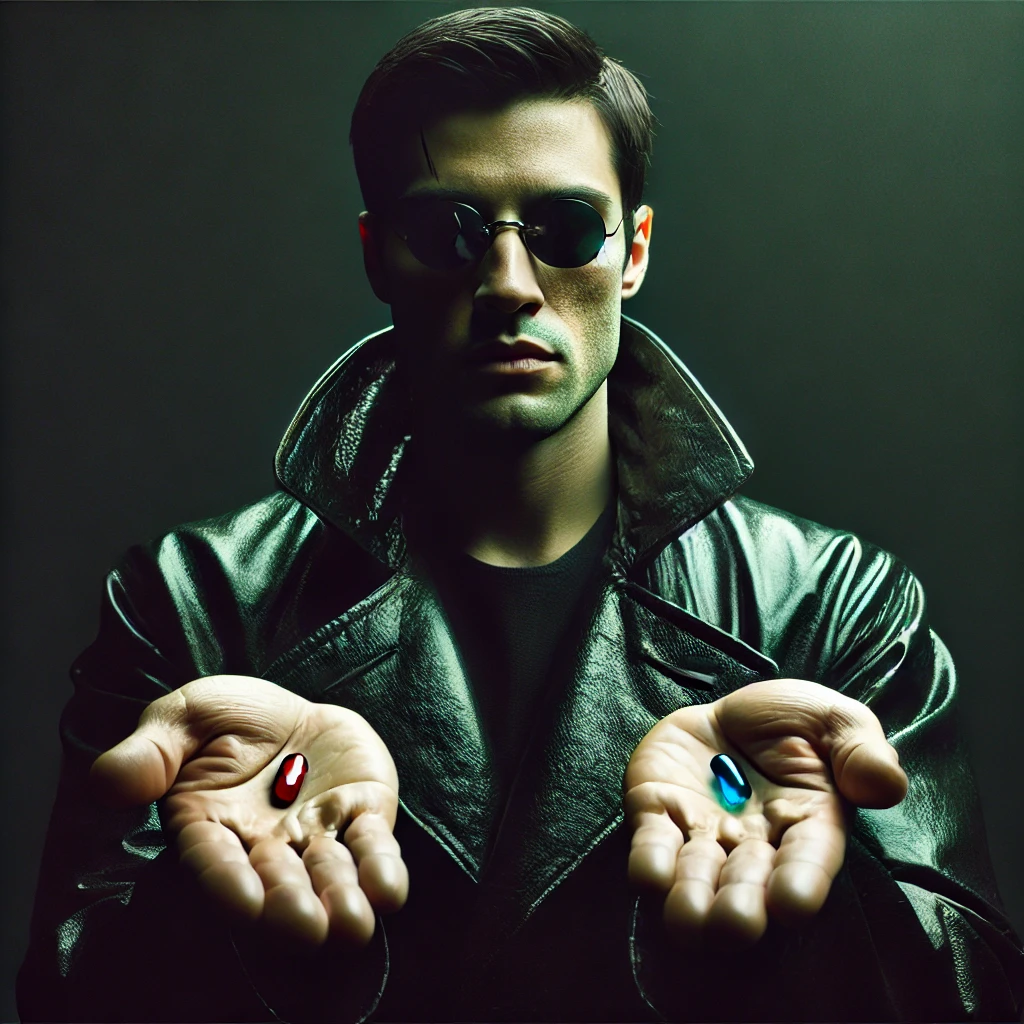
\includegraphics[width=0.618\linewidth]{notneo.png} % 0.618 to złoty podział, bardzo dobra szerokość
	\caption{,,Not Neo'', ChatGPT, 2025}
	\label{rys:notneo}
\end{figure}

Cieszę się, że nadal czytasz ten tekst. A~to znaczy, że wybrane przez Ciebie rozwiązanie to \LaTeX. Jednak nie ma nic za darmo. Jeśli jest to dla Ciebie nowe narzędzie, to musisz je choć trochę poznać.

%%%%%%%%%%%%%%%%%%%%%%%%%%%%%%%%%%%%%%%%%%%%%%%%
\section{Rysunki}
Wydawać by się mogło, że edycja wzorów albo tabel jest największą bolączką początkujących użytkowników \LaTeX{a}. To zaskakujące ale okazuje się, że najwięcej trudności sprawiają rysunki.

Rysunki w~\LaTeX{u} wstawiane są za pomocą polecenia \texttt{includegraphics}. Najczęściej używa się go wewnątrz tak zwanego ,,otoczenia'' \texttt{figure}. To otoczenie pozwala na dodanie podpisu (\texttt{caption}).

Ponadto w~tymże otoczeniu można zdefiniować unikatowy znacznik (\texttt{label}), dzięki któremu można się później w~tekście do tego rysunku odwołać za pomocą \texttt{ref}. Nowo dodany znacznik, jak kilka innych rzeczy w~\LaTeX{u}, może wymagać dwukrotnego uruchomienia kompilacji, gdyż za pierwszym razem \LaTeX{} rejestruje ich obecność a~za drugim już ,,wie'', dokąd mają prowadzić odwołania.

Przykładem jest rysunek~\ref{rys:notneo}, który być może powinien znaleźć się na stronie~\pageref{ch:wstep}, zaraz poniżej słów ,,co wybierasz''. Byłoby fajnie. Jednak tam się nie zmieścił. Dlatego \LaTeX{} przeniósł go na następną stronę. \textbf{To typowe i~normalne zachowanie, z~którym nie należy walczyć.} Dla wielu początkujących użytkowników jest to największa mentalna bariera, którą muszą pokonać. Wynika ona ze złych doświadczeń z~edytorami tekstu, gdzie każdy rysunek trzeba ręcznie ustawić i~zadbać, żeby na pewno wpasował się w~treść na odpowiedniej stronie. A~on i~tak później się przesunie\ldots

\textbf{Dlatego trzeba oduczyć się konieczności ciągłego kontrolowania tak zwanego formatowania.} Celem jest przecież \textit{napisanie} pracy dyplomowej.

Zdarza się, że w~trakcie pisania pracy dyplomowej rysunki nieoczekiwanie ,,fruwają'' gdzieś w~tekście. Czasem \LaTeX{} tworzy z~nich wielką ,,galerię obrazków'' na końcu rozdziału. Nie należy się temu dziwić. Skoro autor tekstu miał intencję zdominować pracę rysunkami, to taki właśnie dokument powstanie. Aby sobie z~tymi problemami radzić, przede wszystkim należy możliwie długo wstrzymać się z~ingerencją w~położenie grafik. Najlepiej zostawić to na sam koniec pisania pracy, gdyż wówczas już ma sens zastosowanie działań takich, jak opisane niżej.

Być może oczekiwany efekt przeniesie przesunięcie otoczenia \texttt{figure} trochę wyżej lub niżej w~źródle \LaTeX{}? Czasem aby odniosło to pożądany skutek należy przenieść je nawet o~kilka akapitów. Trzeba tylko pamiętać o~pustej linii przed i~po nim w~pliku źródłowym.

Można spróbować zmiany sugestii umieszczenia grafiki, czyli h -- \textit{here}, t -- \textit{top}, b -- \textit{bottom}, oraz ewentualnie skorzystanie z~wykrzyknika, który stanowi ,,gorącą prośbę do \LaTeX{a}, żeby się bardziej postarał''.

Skoro rysunki są za duże to może należy je zmniejszyć? Nie każdy rysunek musi zajmować 2/3 szerokości strony. Warto to rozważyć, o~ile zostanie zachowana czytelność ich zawartości. Stopień pisma (wielkość czcionki) wewnątrz rysunku nie może być mniejszy niż wielkość czcionki podpisu pod rysunkiem. Jest to bardzo ważne w~odniesieniu do wykresów i~schematów. Dla treningu możesz spróbować zmniejszyć szerokość rysunku~\ref{rys:notneo} z~0.618 do 0.3 (\texttt{\textbackslash linewidth}) i~zobaczyć, jak wynikowy PDF będzie wyglądał po rekompilacji.

Być może to nie rysunek jest za duży a~treści jest za mało? Do każdego rysunku trzeba odwołać się w~tekście pracy za pomocą \texttt{ref}, tak jak powyżej i~tu ponownie jest odwołanie do rysunku~\ref{rys:notneo}. Zauważ, że \LaTeX{} dba o~spójność numeracji. Każdy rysunek musi być przywołany oraz opisany. Ilość opisującej go treści powinna być porównywalna z~jego powierzchnią. Jeśli nie można wytworzyć takiego opisu a~przecież ,,obraz jest wart tysiąca słów'', to być może ten rysunek niczego do pracy nie wnosi i~po prostu należy go usunąć?

Pozycjonując elementy graficzne a~rysunki w~szczególności, należy zapomnieć o~\underline{złych} poradach w~stylu ,,rysunek powinien pojawić się przed odwołaniem do niego'' albo ,,rysunek powinien być na tej samej stronie, co odwołanie do niego''. Zamiast tego należy wdrożyć swobodniejsze podejście: rysunek powinien być \textbf{możliwie blisko odwołania do niego ale nie bliżej}. Wystarczy, jeśli po ewentualnym wydrukowaniu tekstu czytelnik nie będzie zmuszany do przewracania kartek w~celu znalezienia rysunku, o~którym czyta.

W~\LaTeX{u} praktycznie nie ma ryzyka, że wszystko ,,się rozjedzie'', gdy przesuniemy rysunek. Ewentualne zmiany są też w~pełni odwracalne i~znacznie łatwiejsze, niż w~typowych edytorach tekstu.

Natomiast zdecydowanie \textbf{nie wolno} używać sztuczek, które niszczą sens zautomatyzowanego składu tekstu, czyli takich jak na przykład:
\begin{itemize}
	\item FloatBarrier
	\item pagebreak
	\item newpage
	\item clearpage
\end{itemize}

Powyższe zasady oraz porady można zastosować wobec pozostałych elementów graficznych takich jak tabele i~listingi.

Rysunki rastrowe powinny mieć minimalną rozdzielczość 300 dpi (punktów na cal). Dlatego rysunek zajmujący szerokość strony powinien mieć minimum 1900 pikseli szerokości. Dobry wydruk rastrowy to przynajmniej 600 dpi. Można uzyskać ,,nieskończoną'' rozdzielczość stosując grafikę wektorową. Możliwe jest wyeksportowanie grafik wektorowych do formatu PDF i~użycie ich w~\texttt{includegraphics}.

Inne ,,technikalia'' (\TeX{nikalia}?) wykorzystania \LaTeX{a} są krótko omówione i~zaprezentowane w~dodatku~\ref{app:latex} niniejszego szablonu.

\section{To wspaniale, ale co z~tym wstępem?}

Wstęp pracy dyplomowej powinien zawierać wprowadzenie do zagadnienia na tyle ogólne, żeby również osoba nie mająca wiedzy w~przedstawianym temacie była w~stanie zrozumieć, czego ta praca dotyczy. Opisać należy to, co ,,jest'', a~więc używając czasu teraźniejszego.

Warto we wstępie pokazać zagadnienie za pomocą grafiki (rysunek, schemat, tabela, wykres), aby ułatwić czytelnikowi szybkie rozpoznanie, czego dotyczy dana praca.

Warto posłużyć się odnośnikami bibliograficznymi do źródeł o~niskim progu wymagań -- na przykład czasopism popularnonaukowych lub branżowych.

\textbf{Niezbędnym elementem wstępu jest przedstawienie celu pracy.} Najprościej zacząć zdanie od słów ,,celem pracy jest''. Ponadto można przedstawić cele szczegółowe, założenia pracy, zaplanowane etapy realizacji badań i~innych działań, które będą podjęte w~ramach realizacji pracy dyplomowej dla osiągnięcia jej głównego celu.

Określając powyższe aspekty pracy warto pamiętać, że w~ramach pracy inżynierskiej można podejmować działania
projektowe, technologiczne, organizacyjne i~badawcze. Praca inżynierska powinna przedstawiać weryfikację poprawności uzyskanego rezultatu. Natomiast praca magisterska \textbf{musi} dodatkowo zawierać ,,element badawczy'' a~więc pod wieloma względami powinna stać na wyższym poziomie niż praca inżynierska.

Jeśli omówienie celu pracy i~elementów pokrewnych jest dość długie to może stanowić podrozdział ,,Wstępu''. Aczkolwiek ,,Wstęp'' jako całość raczej nie powinien być tak długi, by wymagał większej liczby podrozdziałów. Teoretyczne podstawy pracy powinny zostać dokładniej przedstawione w~kolejnym rozdziale.
